Analogous to the SVT the ECal DAQ is close to that described for HPS in Sec.~\ref{sec:fadc_daq}. 
The signals from the ECal modules are sent to a signal splitter. One of the outputs of the splitter is fed to a 
discriminator that also has an internal scaler, and then to a TDC channel. The other output is sent to the 
JLab FADC250 VXS module, see Figure \ref{fig:testrun_fadc}. 
\begin{figure}[]
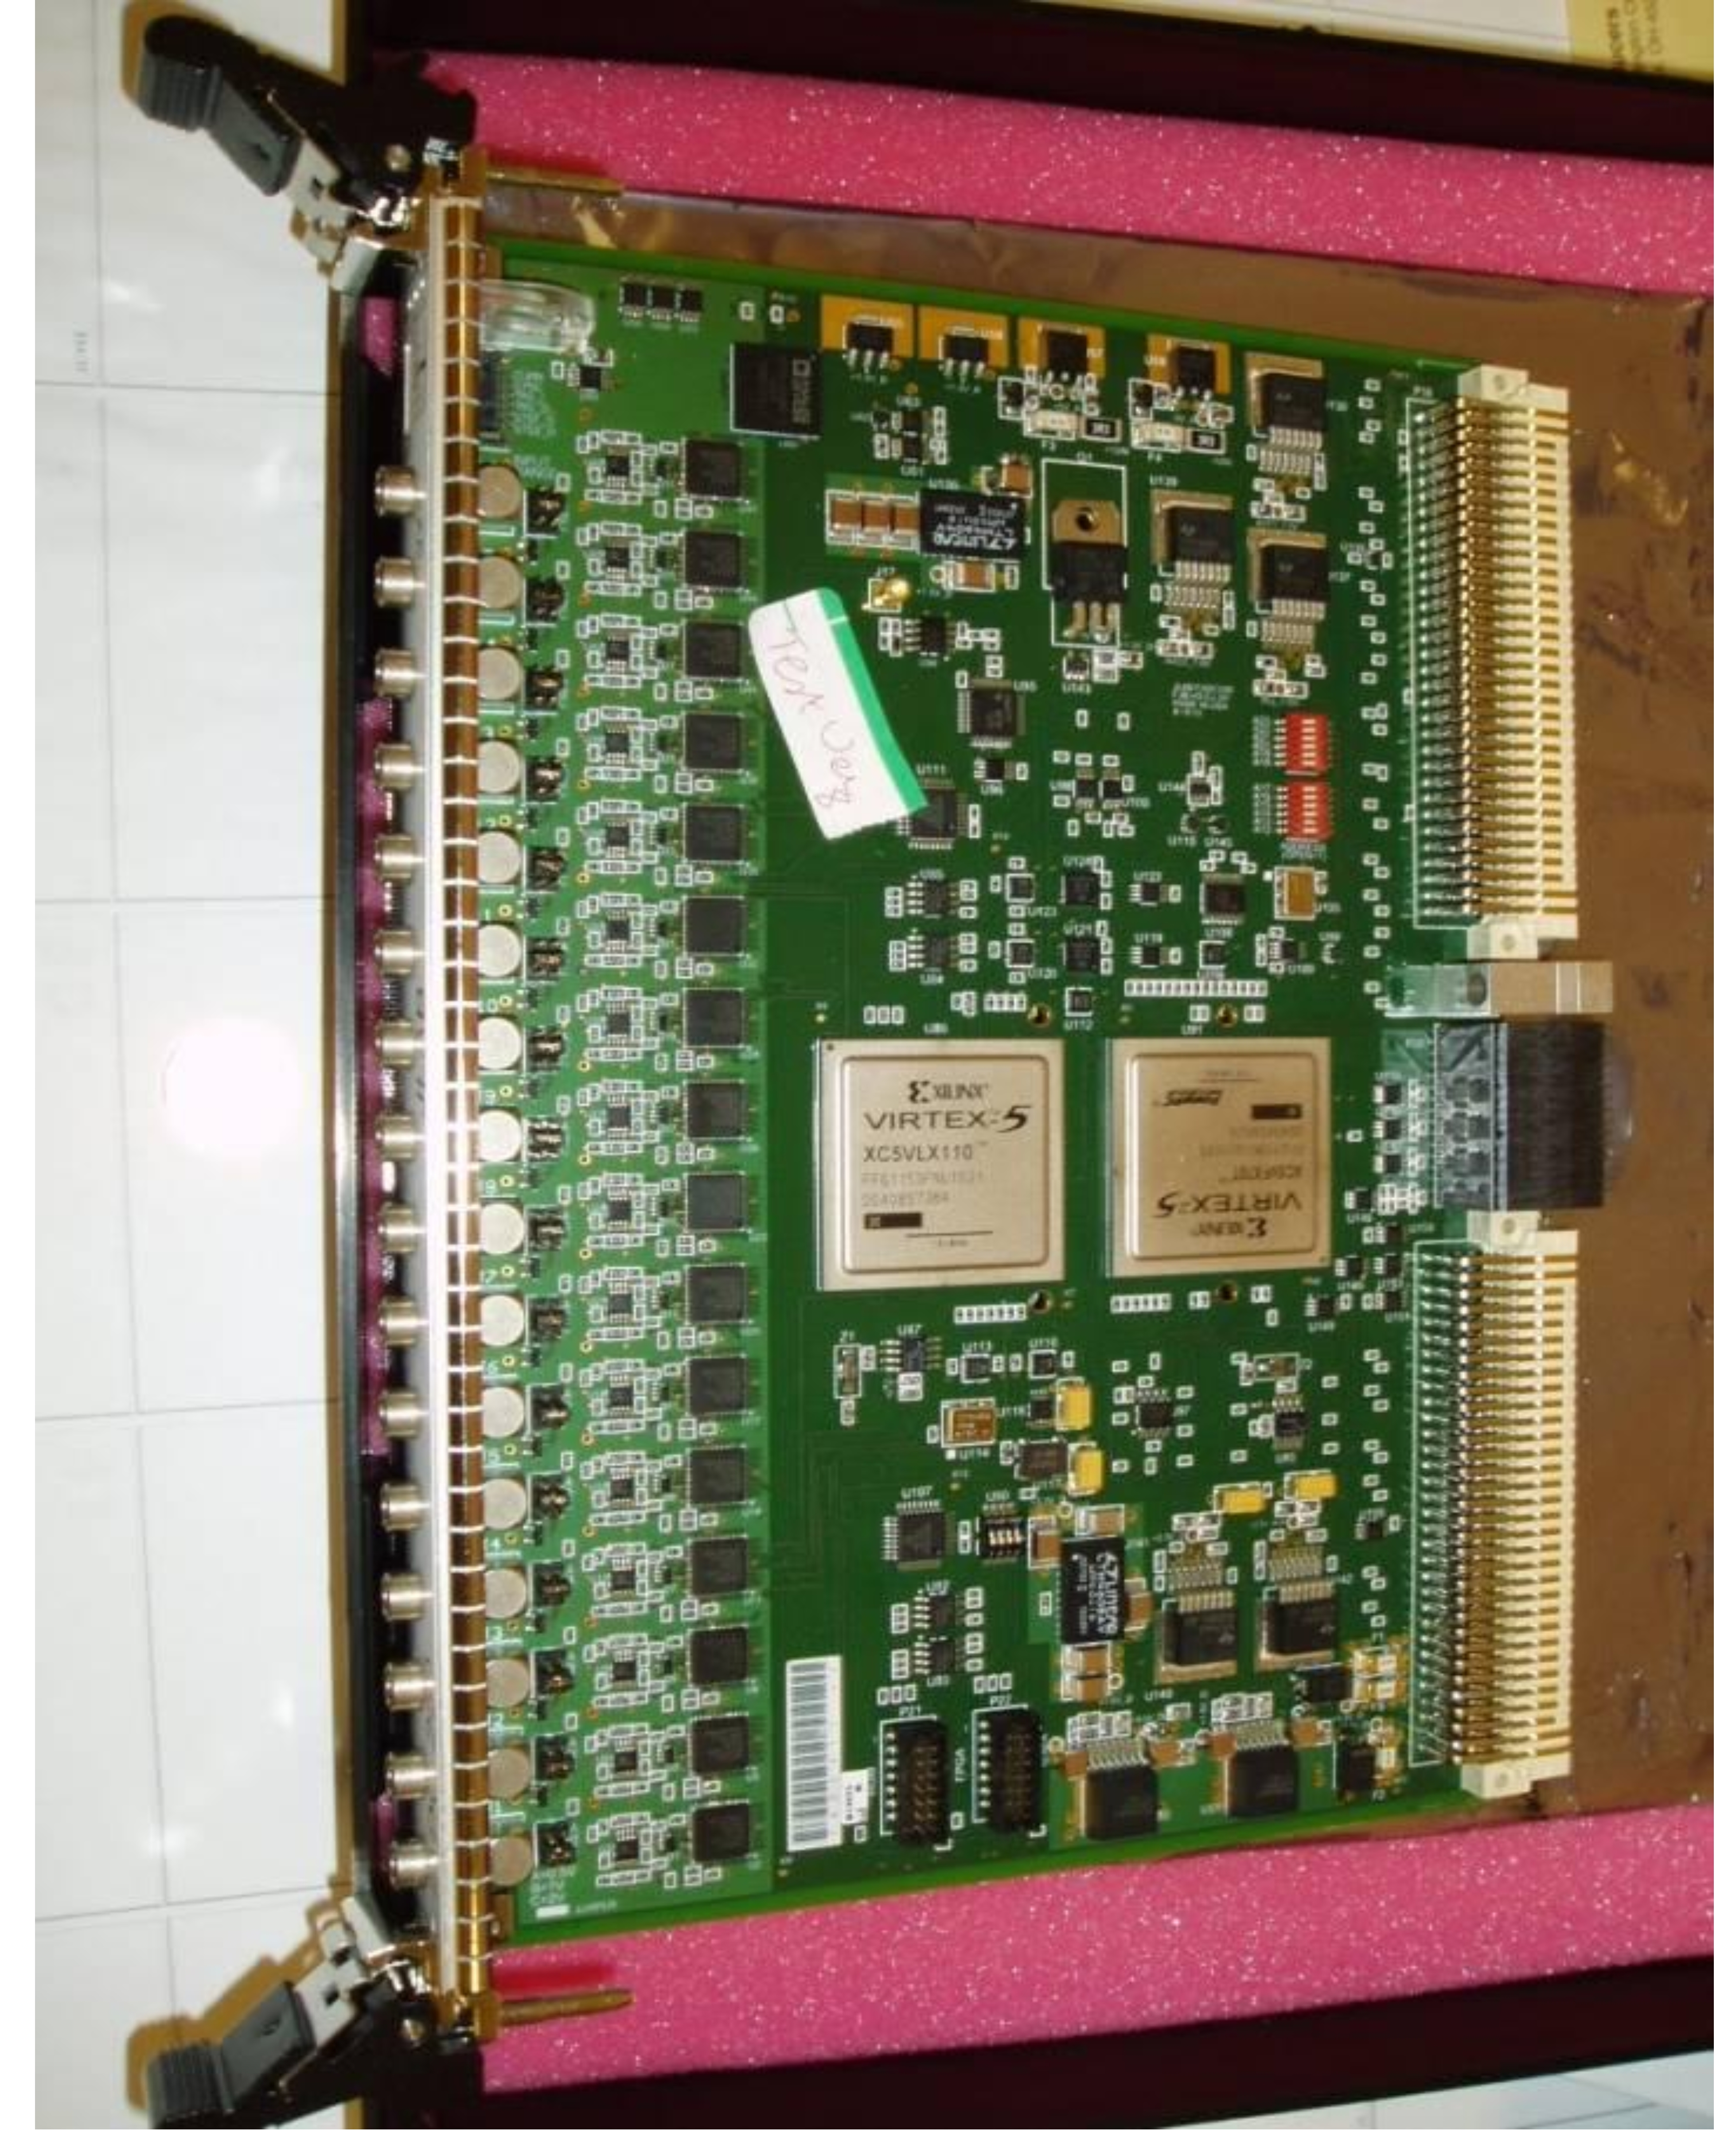
\includegraphics[scale=0.5]{test2012/daq/FADC250_Photo_001.jpg}
\caption{\small{FADC250 VXS module.}}\label{fig:testrun_fadc}
\end{figure}
Two FADC VXS crates are required to 
accommodate the two halves of the ECal. The trigger, described in more details below in 
Sec.~\ref{sec:testrun_trigger}, is based on FADC information and includes a cluster finding algorithm 
using FPGA modules. With the FADCs based system, the energy of clusters used to make a trigger 
decision is determined at the crate level. 
